\chapter{Made in France} 
\label{sec:mif}
\lstset{style=6502Style}
\begin{figure}[H]
    \centering
      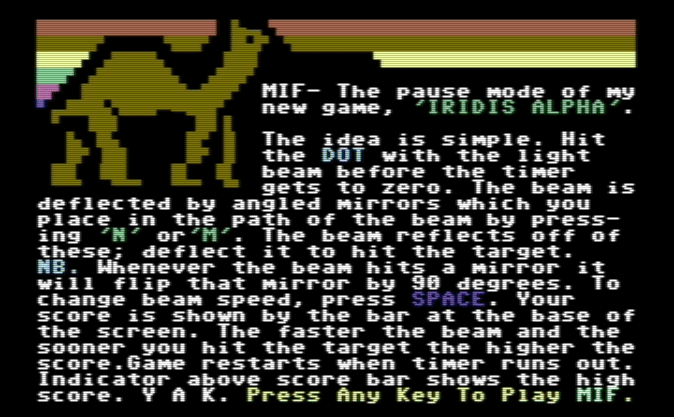
\includegraphics[width=10cm]{src/mif/mif.png}%
\caption{Splash screen for the version of 'Made in France' released on Compunet.}
\end{figure}

I must admit I don't find this pause-mode mini-game of much interest in its own right. I initially
wondered if Jeff Minter had inadvertently invented a precursor to 'Snake', a text-based game that
was once ubiqitous thanks to its inclusion on Nokia mobile phones in the 1990s, but it turns out that
Snake dates back to at least 1976 when the concept first appeared in an arcade game called 'Blockade'.

Perhaps the most noteworthy thing about 'Made in France' (MIF) is how many times Minter has made and remade it. His very
first attempt at the format was one of his earliest games. 'Deflex' was coded in 1981 while he was in college and had access to the 
computer science department's Commodore PET. Viewed side by side it's obvious that one is a slightly more colorful
remake of the other.

\begin{figure}[H]
  {
    \setlength{\tabcolsep}{3.0pt}
    \setlength\cmidrulewidth{\heavyrulewidth} % Make cmidrule = 
	\centering
	\begin{subfigure}{0.5\textwidth}
    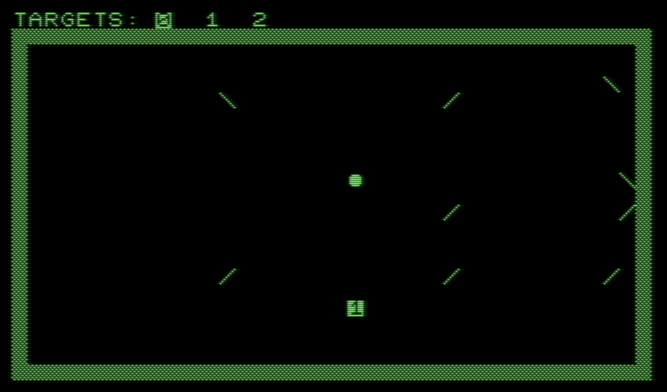
\includegraphics[width=6cm]{src/mif/deflex.png}%
	\end{subfigure}
	\begin{subfigure}{0.5\textwidth}
      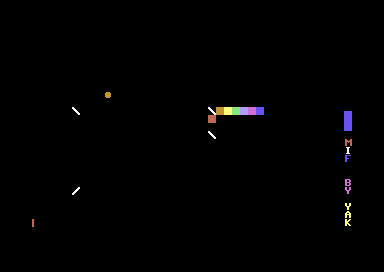
\includegraphics[width=6cm]{src/mif/mif_game.png}%
	\end{subfigure}
  }

\caption{'Deflex' on the left, 'Made in France' on the right.}
\end{figure}

MIF meanwhile was coded while on a ski holiday in France during the making of Iridis Alpha. Minter lugged his development kit on
holiday to the Alps and continued work on Iridis Alpha between time on the slopes and in a couple of evenings remade Deflex into
MIF. He shared this version on Compunet prior to the release of Iridis Alpha and the version that features in the game is unchanged
from that original version.

The gameplay of Deflex and MIF has only a couple of differences. In MIF the player is on a timer and dies if they fail to
complete the level before it elapses.

\begin{figure}[H]
  {
    \setlength{\tabcolsep}{3.0pt}
    \setlength\cmidrulewidth{\heavyrulewidth} % Make cmidrule = 
	\centering
	\begin{subfigure}{0.5\textwidth}
      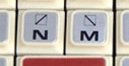
\includegraphics[width=6cm]{src/mif/pet_nm.jpg}%
	\end{subfigure}
	\begin{subfigure}{0.5\textwidth}
      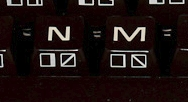
\includegraphics[width=6cm]{src/mif/c64_nm.jpg}%
	\end{subfigure}
  }
\caption{ The controls seem unintuitive to a player using a C64 emulator. Why use 'M' and 'N' for placing paddles? The answer lies in the PET
and C64 keyboard layouts: the 'm' and 'n' keys each bear the paddle glyphs.
}
\end{figure}

\subsubsection{Main Loop}
The code for MIF comes in at a relatively light 900 or so lines of 6502
assembler. The main loop of the game is primarily concerned with detecting key
presses to enter into the DNA mini-game, see
\hyperref[sec:dna]{\textcolor{blue}{A Pause Mode for Your Pause Mode}} or exit
back to Iridis Alpha itself.

\begin{lstlisting}
MIF_RunUntilPlayerUnpauses   
    JSR MIF_InitializeProgressBar
    JSR MIF_DrawCountdownBarAndCredit
    JSR MIF_UpdateProgressBar
    JSR MIF_SetUpInterruptHandler
MIF_MainLoop
    LDA lastKeyPressed
    CMP #$40 ; 'No key pressed'
    BNE MIF_MainLoop

    LDA #$00
    STA $D015    ;Sprite display Enable

    ; Maybe Exit Back to Game
MaybeExitBackToGame
    LDA lastKeyPressed
    CMP #$04 ; F1
    BNE MaybeAsteriskPressed
    ;F1 was pressed, so exit MIF back to game.
    RTS 

MaybeAsteriskPressed
    CMP #$31; '*' Pressed
    BNE MaybeLaunchNewGame

    ; If '*' was pressed, launch DNA.
MIF_DoubleCheckKeyPress
    LDA lastKeyPressed
    CMP #$40 ; 'No key pressed'
    BNE MIF_DoubleCheckKeyPress

    ; Launch DNA
    LDA #$01
    STA mifDNAPauseModeActive
    JSR EnterMainTitleScreen

    ; Relaunch MIF when player exits DNA.
    JMP LaunchMIF

MaybeLaunchNewGame
    LDA mifGameOver
    BEQ MaybeExitBackToGame
    JMP LaunchMIF
\end{lstlisting}

The actual gameplay is handled from an interrupt once per frame.

\begin{lstlisting}
MIF_InterruptHandler   
    LDA $D019    ;VIC Interrupt Request Register (IRR)
    AND #$01
    ; Limits the updates to once per frame.
    BNE PerformGamePlayUpdates
    PLA 
    TAY 
    PLA 
    TAX 
    PLA 
    RTI 

PerformGamePlayUpdates
    JSR UpdateSnakePositionAndCheckInput
    JSR MIF_UpdateCountdownBar
    JSR MIF_PlaySound
    JSR MIF_UpdateTarget
    LDA #$01
    STA $D019    ;VIC Interrupt Request Register (IRR)
    STA $D01A    ;VIC Interrupt Mask Register (IMR)
    LDA #$FE
    STA $D012    ;Raster Position
    JMP $EA31
\end{lstlisting}


